\documentclass{article}
\usepackage{civ}

\title{CIV102: Problem Set \#4}
\author{QiLin Xue \\ \href{mailto:qilin.xue@mail.utoronto.ca}{qilin.xue@mail.utoronto.ca} \\ TA: Michel}
\date{\today}
\usepackage{mathrsfs}
\usetikzlibrary{arrows}
\usepackage{siunitx}
\usepackage{wasysym}
\usetikzlibrary{calc}
\usepackage{xcolor}
\setlength\parindent{0pt}

\begin{document}
\maketitle
\section{Problem One}
\textbf{(a)} Let us draw the free body diagram of three members: $CDE$, $EBH$, and $AB$., as well as the weight $W$. We are able to mostly ignore the left side of the tong by using symmetry. The forces acting on the right side is identical to the forces acting on the left side, except with the horizontal component flipped.
\begin{center}
    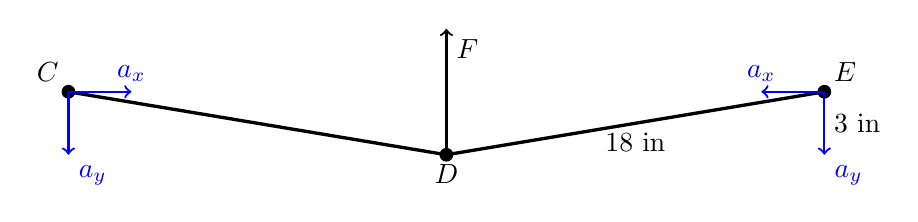
\begin{tikzpicture}[scale=0.8]
        \coordinate (C) at (-6,1);
        \coordinate (D) at (0,0);
        \coordinate (E) at (6,1);
        \draw[fill=black] (C) circle (0.1) node[above left] {$C$};
        \draw[fill=black] (D) circle (0.1) node[below] {$D$};
        \draw[fill=black] (E) circle (0.1) node[above right] {$E$};
        \draw[very thick] (D) -- (E);
        \draw[very thick] (D) -- (C);

        \draw[dotted] (D) -- (E) node[midway,below] {$18\text{ in}$};
        \draw[dotted] (E) -- (D -| E) node[midway,right] {$3\text{ in}$};
        \draw[thick,->] (D) -- ++(0,2) node[below right] {$F$};
        \draw[thick,->,color=blue] (E) -- ++(0,-1) node[below right] {$a_y$};
        \draw[thick,->,color=blue] (E) -- ++(-1,0) node[above] {$a_x$};
        \draw[thick,->,color=blue] (C) -- ++(0,-1) node[below right] {$a_y$};
        \draw[thick,->,color=blue] (C) -- ++(1,0) node[above] {$a_x$};
    \end{tikzpicture}
\end{center}
We can write down one force balance equation, summing up forces in the vertical direction to get:
\begin{equation}
    \sum F_y = 0 \implies a_y=\frac{F}{2}
    \label{eq:eq1}
\end{equation}
Since $DE$ is a thin rod, the compression forces act along the rod. Therefore, we demand that:
\begin{equation}
    \frac{a_y}{a_x}=\frac{3}{\sqrt{18^2-3^2}}=0.169
    \label{eq:2}
\end{equation}
We can also draw a free body diagram for member $EBH$.
\begin{center}
    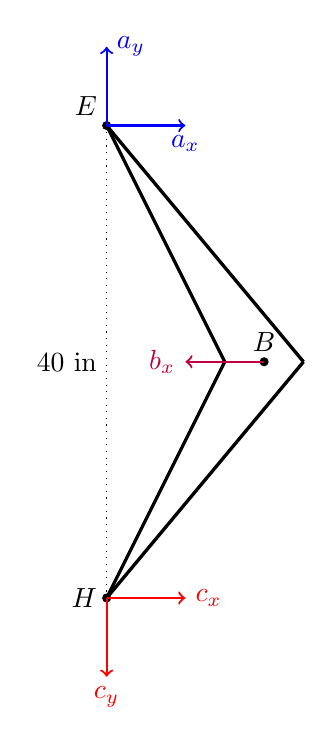
\begin{tikzpicture}[scale=0.5]
        \coordinate (E) at (6,1);
        \coordinate (B) at (10,-5);
        \coordinate (H) at (6,-11);

        \draw[fill=black] (E) circle (0.1) node[above left] {$E$};
        \draw[fill=black] (B) circle (0.1) node[above] {$B$};
        \draw[fill=black] (H) circle (0.1) node[left] {$H$};

        \draw[very thick] (E) -- (9,-5);
        \draw[very thick] (E) -- (11,-5);
        \draw[very thick] (H) -- (9,-5);
        \draw[very thick] (H) -- (11,-5);
        
        \draw[thick,->,color=blue] (E) -- ++(0,2) node[right] {$a_y$};
        \draw[thick,->,color=blue] (E) -- ++(2,0) node[below] {$a_x$};
        \draw[thick,->,color=red] (H) -- ++(0,-2) node[below] {$c_y$};
        \draw[thick,->,color=red] (H) -- ++(2,0) node[right] {$c_x$};
        \draw[thick,->,color=purple] (B) -- ++(-2,0) node[left] {$b_x$};
        \draw[dotted] (E) -- (H) node[midway,left] {$40\text{ in}$};
    \end{tikzpicture}
\end{center}
We can write down three equations: two to balance forces in the horizontal and vertical directions:
\begin{align}
    \sum F_x = 0 &\implies a_x+c_x=b_x    \label{eq:eq3}
    \\ 
    \sum F_y = 0 &\implies a_y=b_y
    \label{eq:eq4}
\end{align}
Here, we have set $b_y=0$ since the tension force acting in the member $AB$ also acts along the direction of the rod. Balancing moments about point $E$, we get:
\begin{equation}
    \sum M_\text{about E}=0 \implies b_x\left(\frac{EH}{2}\right)=c_x\left(EH\right) \implies b_x=2c_x
    \label{eq:eq5}
\end{equation}
% We don't know the horizontal distance $Eb_x$ between point $E$ and point $B$, so it would be convenient for us if $b_y=0$. This is actually the case, and we can prove this by drawing the FBD for $AB$:
% \begin{center}
%     \begin{tikzpicture}[scale=0.5]
%         \coordinate (A) at (-10,-5);
%         \coordinate (B) at (10,-5);

%         \draw[fill=black] (A) circle (0.1) node[above] {$A$};
%         \draw[fill=black] (B) circle (0.1) node[above] {$B$};
%         \draw[very thick] (B) -- (A);

%         \draw[thick,->,color=purple] (B) -- ++(0,-2) node[below] {$b_y$};
%         \draw[thick,->,color=purple] (B) -- ++(2,0) node[below] {$b_x$};
%         \draw[thick,->,color=purple] (A) -- ++(0,-2) node[below] {$b_y$};
%         \draw[thick,->,color=purple] (A) -- ++(-2,0) node[below] {$b_x$};
%     \end{tikzpicture}
% \end{center}
% We see that for every $b_x$, the horizontal force will cancel each other out. To have a net force of zero in the vertical direction though, we must demand $b_y=0$.
Finally, we can draw the FBD of the weight:
\begin{center}
    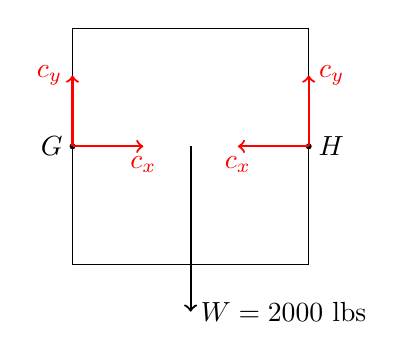
\begin{tikzpicture}[scale=0.3]
        \coordinate (G) at (-5,0);
        \coordinate (H) at (5,0);
        \draw[] (-5,5) rectangle (5,-5);
        \draw[fill=black] (G) circle (0.1) node[left] {$G$};
        \draw[fill=black] (H) circle (0.1) node[right] {$H$};

        \draw[thick,->] (0,0) -- (0,-7) node[right] {$W=2000\text{ lbs}$};
        \draw[thick,->,color=red] (H) -- ++(0,3) node[right] {$c_y$};
        \draw[thick,->,color=red] (H) -- ++(-3,0) node[below] {$c_x$};
        \draw[thick,->,color=red] (G) -- ++(0,3) node[left] {$c_y$};
        \draw[thick,->,color=red] (G) -- ++(3,0) node[below] {$c_x$};
    \end{tikzpicture}
\end{center}
Again, for every value of $c_x$, the horizontal forces will be balanced. But in order for the vertical forces to be balanced, then we must have:
\begin{equation}
    \sum F_y=0 \implies c_y = \frac{W}{2}
    \label{eq:eq6}
\end{equation}
We have six equations involving six unknowns: $F,a_x,a_y,b_x,c_x,c_y$, so we can solve for the system. From equation \ref{eq:eq4}, we can compare equations \ref{eq:eq1} and \ref{eq:eq6} to conclude that $F=W$. This conclusion can also be arrived at by balancing the forces acting on the entire system. We can calculate $a_x$ to be:
\begin{equation}
    a_x = \frac{a_y}{0.169}=\frac{W}{2(0.169)} = 5920 \text{ lbs}
    \label{eq:}
\end{equation}
From equation \ref{eq:eq3} and \ref{eq:eq5}, we can calculate $c_x$ to be:
\begin{equation}
    a_x+c_x=2c_x \implies a_x=\boxed{c_x=5.92 \times 10^3 \text{ lbs}}
    \label{eq:}
\end{equation}
and therefore:
\begin{equation}
    b_x = 2a_x = \frac{W}{0.169} = \boxed{11.83 \times 10^3 \text{ lbs}}
    \label{eq:}
\end{equation}

\newpage
\section{Problem Two}
We can begin by drawing the free body diagram of member $BCD$:
\begin{center}
    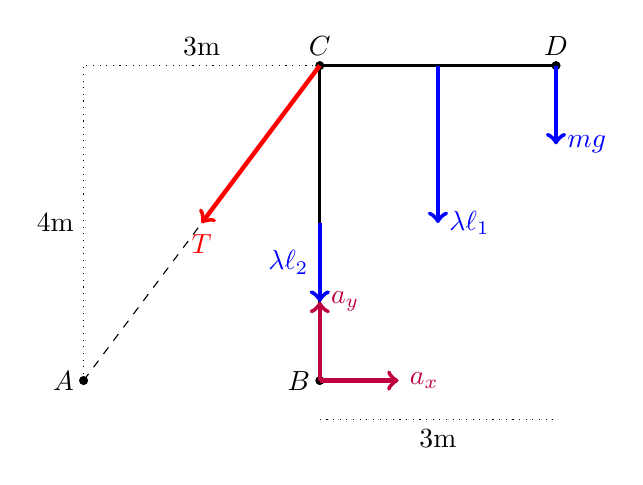
\begin{tikzpicture}
        \coordinate (B) at (3,0);
        \coordinate (C) at (3,4);
        \coordinate (D) at (6,4);
        \coordinate (A) at (0,0);

        \draw[fill=black] (A) circle (0.05) node[left] {$A$};
        \draw[fill=black] (B) circle (0.05) node[left] {$B$};
        \draw[fill=black] (C) circle (0.05) node[above] {$C$};
        \draw[fill=black] (D) circle (0.05) node[above] {$D$};

        \draw[dotted] (A) -- (A |- C) node[midway,left] {$4\si{\meter}$};
        \draw[dotted] (C) -- (A |- C) node[midway,above] {$3\si{\meter}$};
        \draw[dotted] (3,-0.5) -- (6,-0.5) node[midway,below] {$3\si{\meter}$};
        \draw[dashed] (A) -- (C);
        \draw[very thick] (B) -- (C);
        \draw[very thick] (C) -- (D);
        
        \draw[ultra thick,color=blue,->] (D) -- ++(0,-1) node[right] {$mg$};
        \draw[ultra thick,color=blue,->] ($ (C) !.5! (D)$) -- ++(0,-2) node[right] {$\lambda\ell_1$};
        \draw[ultra thick,color=blue,->] ($ (C) !.5! (B)$) -- ++(0,-1) node[midway,left] {$\lambda\ell_2$};

        \draw[ultra thick,color=red,->] (C) -- ($ (C) !.5! (A)$) node[below] {$T$};
        \draw[ultra thick,color=purple,->] (B) -- ++(0,1) node[right] {$a_y$};
        \draw[ultra thick,color=purple,->] (B) -- ++(1,0) node[right] {$a_x$};
    \end{tikzpicture}
\end{center}
where $m=200\si{\kilo\gram}$ is the mass of the sign and $\lambda=1\si{\kilo\newton\per\meter}$ is the linear weight density of the frame. We can balance moments about $B$ to get:
\begin{equation}
    \sum M_\text{about B} = 0 \implies mg(\ell_1)+\lambda\ell_1\left(\frac{\ell_1}{2}\right) = T\frac{\ell_1}{\sqrt{\ell_2^2+\ell_1^2}}\left(\ell_2\right) 
    \label{eq:}
\end{equation}
where $\ell_1=3\si{\meter}$ and $\ell_2=4\si{\meter}$ respectively. Substituting in numbers and solving for $T$ gives:
\begin{equation}
    5886+4500=\frac{3}{5}T(4) \implies \boxed{T=4.33\si{\kilo\newton}}
    \label{eq:}
\end{equation}
Balancing forces in the vertical direction, we have:
\begin{equation}
    \sum F_y=0 \implies \frac{4}{5}T+\lambda(\ell_1+\ell_2)+mg=a_y \implies \boxed{a_y=12.42\si{\kilo\newton}}
    \label{eq:}
\end{equation}
and balancing forces in the horizontal direction, we have:
\begin{equation}
    \sum F_x=0 \implies \frac{3}{5}T=a_x \implies \boxed{a_x=2.60\si{\kilo\newton}}
    \label{eq:}
\end{equation}
such that the reaction force at point $B$ is:
\begin{equation}
    |\vec{a}|=\sqrt{a_x^2+a_y^2}=\boxed{12.69\si{\kilo\newton}}
    \label{eq:}
\end{equation}
The stress in the cable as a function of the diameter $d$ is given by:
\begin{equation}
    \sigma = T\left(\frac{4}{\pi d^2}\right) = \frac{800\si{\mega\pascal}}{2} \implies d = \sqrt{\frac{8T}{\pi \cdot 800\si{\mega\pascal}}} = 3.711\si{\milli\meter}
    \label{eq:}
\end{equation}
We round up to get $\boxed{d=3.72\si{\milli\meter}}$ to ensure a FOS of at least $2$.
\newpage

\section{Problem Three}
Let's lay out an overall plan first. There are four unknowns: the tension in the rope, $F_x$ and $F_y$ from the pivot, and the normal interaction $N$ between the weight and the beam. We thus need four equations. We can generate three equations by balancing horizontal and vertical forces, as well as balancing moments. We can generate our fourth equation by doing a force balance on the weight. Let's draw the free body diagram of the beam:
\begin{center}
    \begin{tikzpicture}[scale=2]
        \coordinate (A) at (0,0);
        \coordinate (B) at (1,0);
        \coordinate (C) at (3,0);
        \coordinate (D) at (5,0);

        \draw[fill=black] (A) circle (1pt) node[below left] {$A$};
        \draw[fill=black] (B) circle (1pt) node[below left] {$B$};
        \draw[] (1.25,0.1) node[] {$\theta$};
        \draw[fill=black] (C) circle (1pt) node[below left] {$C$};
        \draw[fill=black] (D) circle (1pt) node[below left] {$D$};

        \draw[thick] (A) -- (B);
        \draw[thick] (B) -- (C);
        \draw[thick] (C) -- (D);

        \draw[dotted,<->] (0,-2) -- (1,-2) node[midway,below] {$1\si{\meter}$};
        \draw[dotted,<->] (1,-2) -- (3,-2) node[midway,below] {$2\si{\meter}$};
        \draw[dotted,<->] (3,-2) -- (5,-2) node[midway,below] {$2\si{\meter}$};
        \draw[dotted,<->] (C) -- (3,1.5) node[midway,right] {$1.5\si{\meter}$};

        \draw[color=blue,->,very thick] (B) -- ++(2,1.5) node[right] {$T$};
        \draw[color=red,->,very thick] (C) -- ++(0,-1) node[right] {$N$};
        \draw[color=red,->,very thick] (2.5,0) -- ++(0,-1.5) node[left] {$\lambda L$};
        \draw[color=black,->,very thick] (D) -- ++(0,0.5) node[right] {$A_y$};
        \draw[color=black,->,very thick] (D) -- ++(-0.5,0) node[below] {$A_x$};

    \end{tikzpicture}
\end{center}
Note that the angle given here is $\theta=\arctan\left(\frac{4}{3}\right)$. Balancing forces in the vertical ($y$) and horizontal directions ($x$) gives:
\begin{align}
    \sum F_y &= 0 \implies \frac{3}{5}T+A_y=\lambda L + N \label{eq:3-1}\\
    \sum F_x &= 0 \implies \frac{4}{5}T=A_x\label{eq:3-2}
\end{align}
and balancing moments about $D$ gives:
\begin{equation}
    \sum M = 0 \implies 4\left(\frac{3}{5}T\right)=2.5(\lambda L)+ 2(N)
    \label{eq:3-3}
\end{equation}
We can also balance forces on the weight $W$:
\begin{center}
    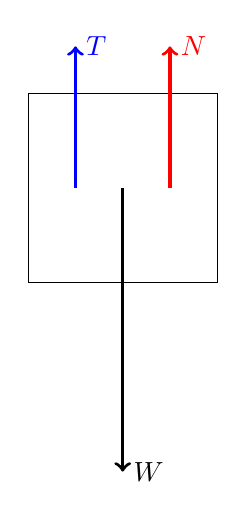
\begin{tikzpicture}[scale=0.6]
        \draw[] (0,0) rectangle (4,4);
        \draw[->,very thick,blue] (1,2) -- ++(0,3) node[right] {$T$};
        \draw[->,very thick,red] (3,2) -- ++(0,3) node[right] {$N$};
        \draw[->,very thick,black] (2,2) -- ++(0,-6) node[right] {$W$};
    \end{tikzpicture}
\end{center}
to get:
\begin{equation}
    T = W - N
    \label{eq:3-4}
\end{equation}
As a recap, $\lambda=8\si{\kilo\newton\per\meter}$ is the linear weight density of the beam, and $T$ is the tension force in the cable. We can substitute $T$ into equation \ref{eq:3-3} to solve for $N$:
\begin{equation}
    \frac{12W}{5}-\frac{12N}{5}=\frac{5}{2}\lambda L + 2N \implies N = \frac{6}{11}W-\frac{25}{44}\lambda L \implies \boxed{N=4.55\si{\kilo\newton}}
    \label{eq:}
\end{equation}
Substituting this back into equation \ref{eq:3-4} gives us:
\begin{equation}
    T = W-\left(\frac{6}{11}W-\frac{25}{44}\lambda L\right) = \frac{25}{44}\lambda L + \frac{5}{11}W \implies \boxed{T=45.5\si{\kilo\newton}}
    \label{eq:}
\end{equation}
Substituting values of $T$ and $N$ into equations \ref{eq:3-1} and \ref{eq:3-2} gives:
\begin{align}
    A_y = \lambda L + \left(\frac{6}{11}W-\frac{25}{44}\lambda L\right)- \frac{3}{5}\left(\frac{25}{44}\lambda L + \frac{5}{11}W\right) = \frac{1}{11}\lambda L + \frac{3}{11}W &\implies \boxed{A_y=17.27\si{\kilo\newton}} \\ 
    A_x = \frac{4}{5}\left(\frac{25}{44}\lambda L + \frac{5}{11}W\right) = \frac{5}{11}\lambda L + \frac{4}{11}W &\implies \boxed{A_x=36.4\si{\kilo\newton}}
\end{align}

\newpage
\section{Problem Four}
Wow... this assignment is very obsessed with special triangles...

\textbf{(a)} Let us define $\theta_0=\arctan\left(\frac{3}{4}\right)$ be the angle that the diagonal of the rectangle makes with the two shorter sides. Then if the crate rotates by an angle $\theta$, then we can do a moment balance around the pivot. We are assuming that the coefficient of static friction is high enough such that it doesn't slip.
\begin{center}
    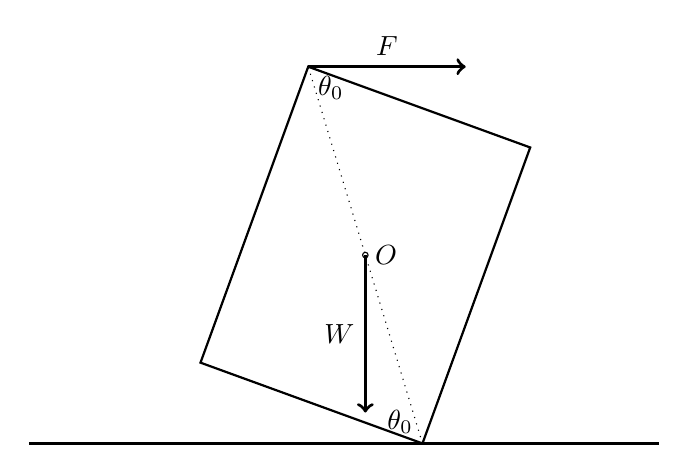
\begin{tikzpicture}
        \draw[thick] (-2,0) -- (6,0);
        \coordinate (A) at (3,0);
        \coordinate (P) at ([rotate around={-20:(3,0)}]0,4);
        \coordinate (O) at ([rotate around={-20:(3,0)}]1.5,2);
        \draw[thick,rotate around={-20:(3,0)}] (0,0) rectangle (3,4);
        \draw[] (O) circle (1pt) node[right] {$O$};
        \draw[very thick, ->] (O) -- ++(0,-2) node[midway,left] {$W$};
        \draw[very thick, ->] (P) -- ++(2,0) node[midway,above] {$F$};
        \draw[dotted] (A) -- (P);
        \node[below right] at (P) {$\theta_0$};
        \node[above left] at (A) {$\theta_0$};
    \end{tikzpicture}
\end{center}
The length of the diagonal is $D=2\si{\meter}$, so the moment due to the force is:
\begin{equation}
    M_\text{horizontal force} = FD\sin(\theta_0+\theta)
    \label{eq:}
\end{equation}
The moment due to gravity is:
\begin{equation}
    M_\text{gravity} = \frac{D}{2}W\cos(\theta_0+\theta)
    \label{eq:}
\end{equation}
These two moments have to cancel each other out, or:
\begin{align}
    F\sin(\theta_0+\theta) &= \frac{W}{2}\cos(\theta_0+\theta) \\ 
    F &= \frac{W}{2}\cot(\theta_0+\theta)
    \label{eq:}
\end{align}
We can plot out the force in kN as a function of the angle rotated, when $\theta_0+\theta=\frac{\pi}{2}$. In the graph below, I have included part of the graph before and after the supposed endpoint. We can physically interpret the part before as: ``If there was no ground, then we needed to exert this amount of force to keep the crate in equilibrium.'' The part after can be interpreted as the force we need to pull on the box to keep it from toppling over.
\begin{center}
    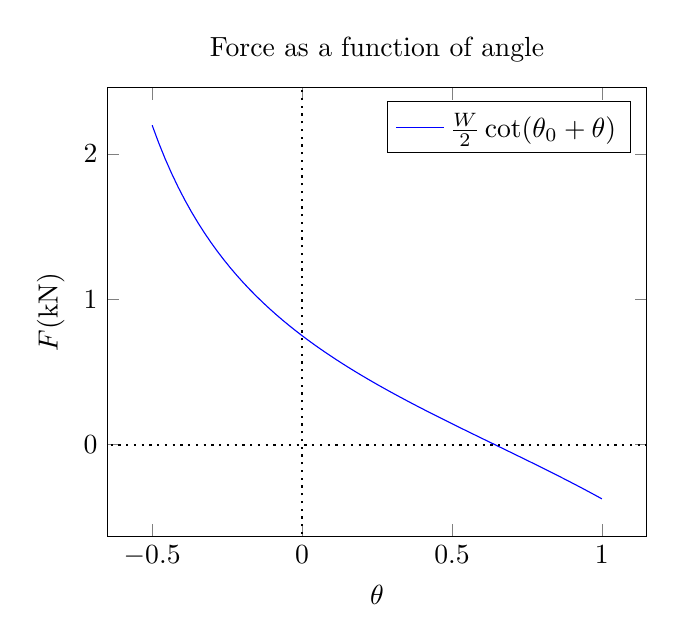
\begin{tikzpicture}
        \begin{axis}[
        title=Force as a function of angle,
        axis lines = box,
        ylabel = $F(\si{\kilo\newton})$,
        xlabel = $\theta$,
        variable = t,
        trig format plots = rad,
        legend pos=north east,
        ]
        \addplot [
            domain=-0.5:1,
            samples=70,
            color=blue,
            ]
            {cos(0.927+x)/sin(0.927+x)};
        \addlegendentry{$\frac{W}{2}\cot(\theta_0+\theta)$}
        \draw[thick,dotted] (-1,0) -- (2,0);
        \draw[thick,dotted] (0,-2) -- (0,6);
        \end{axis}
    \end{tikzpicture}
\end{center}
We can zoom in on the desired region:
\begin{center}
    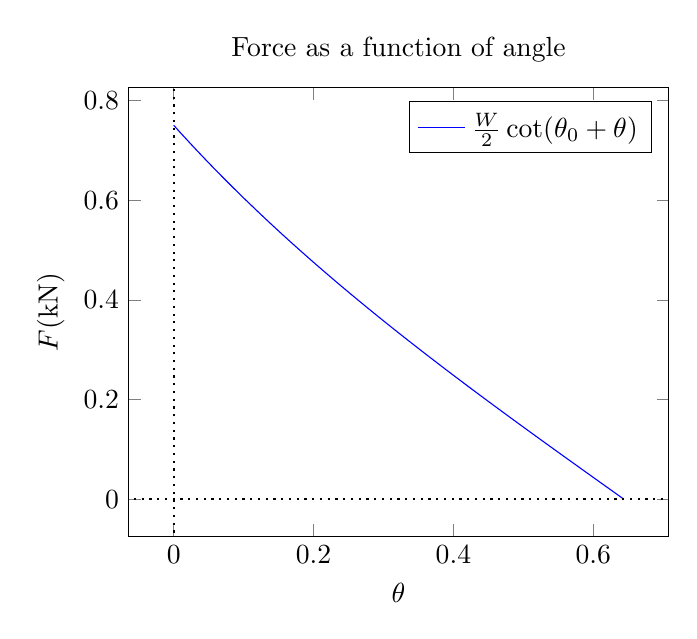
\begin{tikzpicture}
        \begin{axis}[
        title=Force as a function of angle,
        axis lines = box,
        ylabel = $F(\si{\kilo\newton})$,
        xlabel = $\theta$,
        variable = t,
        trig format plots = rad,
        legend pos=north east,
        ]
        \addplot [
            domain=0:0.643,
            samples=70,
            color=blue,
            ]
            {cos(0.927+x)/sin(0.927+x)};
        \addlegendentry{$\frac{W}{2}\cot(\theta_0+\theta)$}
        \draw[thick,dotted] (-0.5,0) -- (2,0);
        \draw[thick,dotted] (0,-1) -- (0,3);
        \end{axis}
    \end{tikzpicture}
\end{center}
Eh, not so interesting. Only comment is that it is monotonically decreasing so that the maximum force occurs when $\theta=0$. We'll use this for the next part.

\textbf{(b)} We essentially we want to maximize the torque. This can be done if the angle between $F$ and the moment arm is $\pi/2$, which can be achieved if we apply a force acting perpendicular to the diagonal.

Thus when performing a moment balance at the time of the maximum force, we get:
\begin{equation}
    D(F) = \left(\frac{D}{2}\cos\theta_0\right)W \implies F = \frac{3W}{10} \implies \boxed{F=0.6\si{\kilo\newton}}
    \label{eq:}
\end{equation}

\newpage
\section{Problem Five}
\textbf{(a)} If there is no wind, then the roller and the pin should share the vertical reaction force equally. If a building has $N$ stories, then the total weight is:
\begin{equation}
    W_\text{total}=NW_\text{grav}w=N(1080\si{\kilo\newton})
    \label{eq:}
\end{equation}
and assuming $h \in {0,4,8,16,...,300}$ the number of stories $N$ is given by $N=\frac{h}{4}$. The weight experienced by the pin is half of this, or:
\begin{equation}
    F_\text{y,pin} = \frac{W_\text{total}}{2} = \frac{h}{8}(1080\si{\kilo\newton}) \implies \boxed{F_\text{y,pin} = (135\si{\kilo\newton\per\meter})h}
    \label{eq:}
\end{equation}
We can plot this:
\begin{center}
    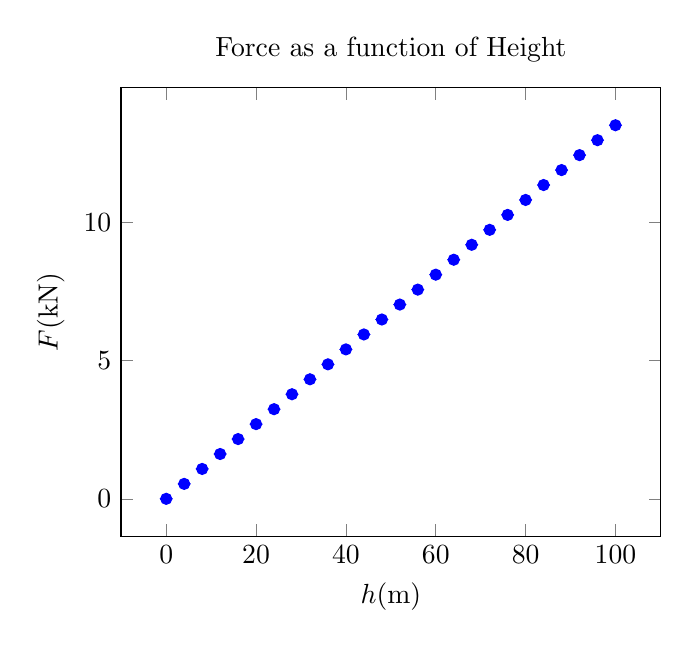
\begin{tikzpicture}
        \begin{axis}[%
        title=Force as a function of Height,
        axis lines = box,
        ylabel = $F(\si{\kilo\newton})$,
        xlabel = $h(\si{\meter})$,
        scatter/classes={%
        a={mark=o,draw=black}}
        ]
        \addplot[color=blue,mark=*,only marks,error bars/.cd,
        y dir=both,y explicit,
        x dir=both,x fixed=0.05,
        error mark=diamond*] coordinates {
            (0	,0)
            (4	,0.54)
            (8	,1.08)
            (12,	1.62)
            (16,	2.16)
            (20,	2.7)
            (24,	3.24)
            (28,	3.78)
            (32,	4.32)
            (36,	4.86)
            (40,	5.4)
            (44,	5.94)
            (48,	6.48)
            (52,	7.02)
            (56,	7.56)
            (60,	8.1)
            (64,	8.64)
            (68,	9.18)
            (72,	9.72)
            (76,	10.26)
            (80,	10.8)
            (84,	11.34)
            (88,	11.88)
            (92,	12.42)
            (96,	12.96)
            (100,	13.5 )
        };
    \end{axis}
        \end{tikzpicture}
\end{center}
\textbf{(b)} We can balance the moments about the roller. The wind acts with a center of force $\frac{2}{3}h$ from the bottom, with a total force of $W_\text{wind,avg}=(\frac{3}{4}\si{\kilo\newton\per\meter})h^2$ for a total moment of:
\begin{equation}
    M_\text{wind} = \left(\frac{1}{2}\si{\kilo\newton\per\meter}\right)h^3
    \label{eq:}
\end{equation}
and the moment due to the vertical force of the pin is:
\begin{equation}
    M_\text{vertical force of pin} = (9\si{\meter})F_\text{y,pin}
    \label{eq:}
\end{equation}
Setting them equal to each other gives:
\begin{equation}
    F_\text{y,pin} = \left(\frac{1}{18}\si{\kilo\newton\per\meter\squared}\right)h^3
    \label{eq:}
\end{equation}
which if plotted out, gives:
\begin{center}
    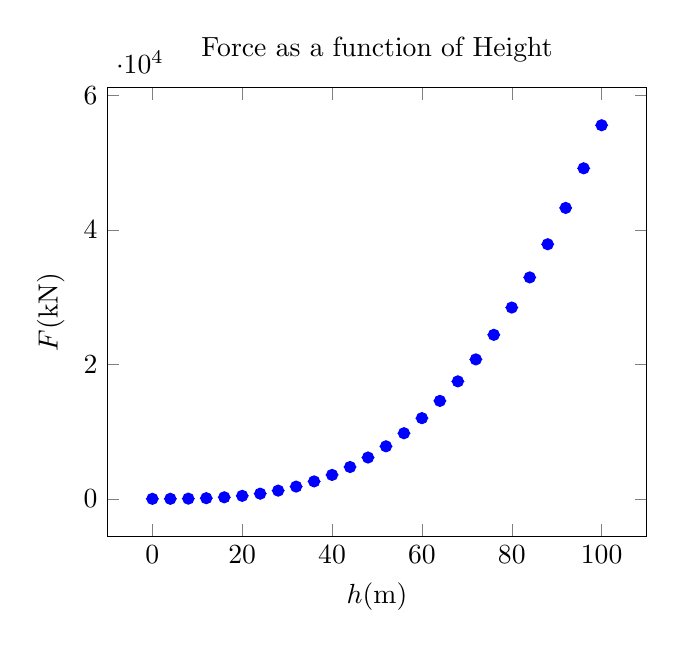
\begin{tikzpicture}
        \begin{axis}[%
        title=Force as a function of Height,
        axis lines = box,
        ylabel = $F(\si{\kilo\newton})$,
        xlabel = $h(\si{\meter})$,
        scatter/classes={%
        a={mark=o,draw=black}}
        ]
        \addplot[color=blue,mark=*,only marks,error bars/.cd,
        y dir=both,y explicit,
        x dir=both,x fixed=0.05,
        error mark=diamond*] coordinates {
            (0	,0)
            (4	,3.555555556)
            (8	,28.44444444)
            (12,	96)
            (16,	227.5555556)
            (20,	444.4444444)
            (24,	768)
            (28,	1219.555556)
            (32,	1820.444444)
            (36,	2592)
            (40,	3555.555556)
            (44,	4732.444444)
            (48,	6144)
            (52,	7811.555556)
            (56,	9756.444444)
            (60,	12000)
            (64,	14563.55556)
            (68,	17468.44444)
            (72,	20736)
            (76,	24387.55556)
            (80,	28444.44444)
            (84,	32928)
            (88,	37859.55556)
            (92,	43260.44444)
            (96,	49152)
            (100,	55555.55556)
        };
    \end{axis}
        \end{tikzpicture}
\end{center}

\textbf{(c)} We do essentially the same thing, but we take into consideration the moment due to gravity:
\begin{equation}
    M_\text{gravity} = W_\text{total} \cdot (4\si{\meter}) = \left(1080\si{\kilo\newton\per\meter}\right)h
    \label{eq:}
\end{equation}
which works in the same direction as the wind, such that:
\begin{equation}
    M_\text{wind}+M_\text{gravity}=M_\text{vertical force of pin} \implies 9F_\text{y,pin} = 1080h + \frac{1}{2}h^3
    \label{eq:}
\end{equation}
When the left side loses contact, then all the vertical force is supported by $F_\text{y,pin}=W_\text{total}$, which gives us:
\begin{equation}
    9(270h)=1080h+\frac{1}{2}h^2 \implies h=51.9\si{\meter}
    \label{eq:}
\end{equation}
which rounds down to $\boxed{12 \text{ stories}}$

\textbf{(d)} No, because the force experienced by the pin increases with $h^3$, so doubling the height causes \textit{at least} an increase in the force of the pin by eight times. To maintain an appropriate factor of safety, I estimate that eight times the reinforcements need to be made and thus have eight times the cost. This is of course only a ballpark estimate.
\end{document}
